% =============================================================================
% SECTION 5 — ANALYSIS
% Core findings only. Full trajectory metrics, action-type distributions,
% the concrete contrast example, no-patch mechanism, and multi-file analysis
% are moved to Appendix~\ref{app:behavior_extra}.
% All trajectory-level statistics are computed from three independent
% evaluation runs of each checkpoint (baseline = R2E-Gym post-training only;
% ours = FIM-Midtrain + R2E-Gym), reported as run-means.
% =============================================================================

\section{Analysis}
\label{sec:analysis}

The previous section established that FIM mid-training improves end-task
metrics. We now ask \emph{how} the resulting agent behaves differently and
\emph{where} along the trajectory the gains accrue, focusing on the two
findings that most directly bear on the motivating hypothesis. Both
analyses are performed on the 14B configuration with R2E-Gym
post-training, comparing the post-training-only baseline (\emph{R2E-Gym})
against our recipe (\emph{FIM-Midtrain $+$ R2E-Gym}). Every
trajectory-level statistic is computed over three independent evaluation
runs of each checkpoint and reported as the run-mean on the
SWE-Bench-Verified test set ($500$ instances per run); the corresponding
analysis on SWE-Bench-Lite, the full action-type distribution, the
no-patch mechanism, and a concrete trajectory contrast are deferred to
Appendix~\ref{app:behavior_extra} and \ref{app:behavior_lite}.

% -----------------------------------------------------------------------------
% Headline behavioral finding: recovery rate
% -----------------------------------------------------------------------------
\subsection{Recovery from Negative Observations}
\label{sec:analysis:recovery}

We define a trajectory as containing a \emph{negative observation} if any
step's tool output matches one of a fixed set of error patterns (stack
traces, ``\texttt{No replacement was performed}'', ``\texttt{SyntaxError}'',
shell errors, etc.; full list in Appendix~\ref{app:algo}). The fraction
of such trajectories is essentially identical between the two checkpoints
($88.8\%$ baseline vs.\ $91.8\%$ ours), so the agents are exposed to
comparable amounts of negative feedback. The \emph{recovery rate}---the
fraction of error-containing trajectories that nevertheless terminate
with a passing patch---rises from $24.8\%$ to $28.8\%$ ($+4.0$~pp, a
$16\%$ relative increase; Table~\ref{tab:behavior_main}). This metric
tracks the precise capability our framing predicts mid-training should
support: continuing productively after an external return contradicts
the model's prior expectation. Mid-training also shifts the agent toward
an iterate-and-verify policy, increasing edits per solved task from
$3.3$ to $7.4$ and trajectory length from $15.1$ to $23.6$ steps;
detailed action-type breakdowns are in
Appendix~\ref{app:behavior_extra}.

% -----------------------------------------------------------------------------
% TABLE — compact summary of the headline metrics
% -----------------------------------------------------------------------------
\begin{table}[h]
\centering
\caption{Headline trajectory-level metrics on SWE-Bench-Verified (14B,
R2E-Gym pipeline), averaged over three independent evaluation runs of
each checkpoint. ``Recovery rate'' is the fraction of trajectories
containing a negative observation that terminate with a passing patch;
``Edits / solved'' is the mean number of \texttt{file\_editor}
operations on solved tasks. Full metrics, including unsolved-trajectory
statistics, action-type distributions, and per-checkpoint output/context
summaries, are in Appendix~\ref{app:behavior_extra}.}
\label{tab:behavior_main}
\small
\setlength{\tabcolsep}{8pt}
\begin{tabular}{lcccc}
\toprule
Setting & Recovery rate (\%) & Edits / solved & Steps / solved & Pass (\%) \\
\midrule
+ R2E-Gym                          & 24.8           & 3.3           & 15.1           & 26.2 \\
\textbf{+ FIM-Midtrain + R2E-Gym}  & \textbf{28.8}  & \textbf{7.4}  & \textbf{23.6}  & \textbf{29.2} \\
\bottomrule
\end{tabular}
\end{table}

% -----------------------------------------------------------------------------
% Closing-loop result: where the gain concentrates
% -----------------------------------------------------------------------------
\subsection{The Gain Concentrates on Multi-Function Reasoning}
\label{sec:analysis:multifn}

The most direct test of our isomorphism argument
(Section~\ref{sec:method:motivation}) is whether mid-training
preferentially helps tasks whose successful resolution requires
reasoning about cross-function dependencies inside a file. We stratify
the $500$ Verified tasks by the shape of the gold patch
(Figure~\ref{fig:patchshape}). On the $88$ tasks whose gold patch
modifies $\ge 2$ functions within a single file, the baseline solves
$13.6\%$ on average and ours solves $22.7\%$, an absolute gain of
$+9.1$~pp---more than $4{\times}$ the gain on the $341$ single-function
tasks ($+2.1$~pp). Per-instance head-to-head on this bucket shows ours
uniquely solves about twice as many tasks as the baseline does. Multi-file
tasks ($n{=}71$) are not differentially helped by mid-training, which we
attribute to a granularity mismatch (our FIM operates within files);
discussion is deferred to Appendix~\ref{app:behavior_extra}.

% -----------------------------------------------------------------------------
% FIGURE — pass rate by gold-patch shape (the multi-function panel only)
% -----------------------------------------------------------------------------
\begin{figure}[h]
\centering
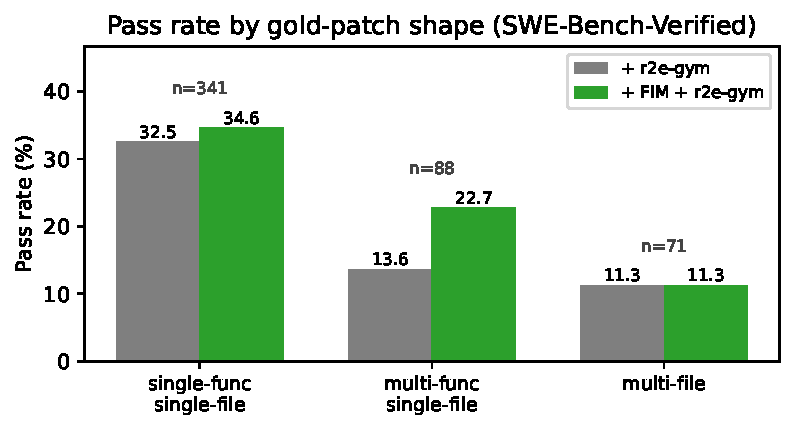
\includegraphics[width=0.62\linewidth]{figs/passrate_by_patchshape_verified.pdf}
\caption{Pass rate on SWE-Bench-Verified ($14$B + R2E-Gym) stratified by
the shape of the gold patch, averaged over three evaluation runs per
checkpoint. The largest absolute gain is on \emph{multi-function
single-file} tasks ($+9.1$~pp), more than $4{\times}$ the gain on
single-function tasks ($+2.1$~pp); multi-file tasks remain hard for both
checkpoints ($\sim\!11.3\%$ each).}
\label{fig:patchshape}
\end{figure}

We read this concentration as a closing-loop confirmation of the
isomorphism argument in Section~\ref{sec:method:motivation}: the slice
where mid-training helps most is precisely the slice where the agent
must follow control- and data-dependencies between caller-callee or
sibling functions inside a file---the same structure exposed by
function-aware FIM masking. A complementary outcome-distribution
breakdown (Figure~\ref{fig:failure_app} in Appendix) shows that the
$+15$-task gain is driven by an order-of-magnitude reduction in
\emph{no-patch} failures alongside small reductions in localization
errors; we interpret the no-patch collapse as a direct consequence of
the FIM training signal, which conditions the model to produce a
non-empty span between the prefix and suffix---a disposition that
survives subsequent post-training.